%% %%%%%%%%%%%%%%%%%%%%%%%%%%%%%%%%%%%%%%%%%%%%%%%%%
%% Template for a conference paper, prepared for the
%% Food and Resource Economics Department - IFAS
%% UNIVERSITY OF FLORIDA
%% %%%%%%%%%%%%%%%%%%%%%%%%%%%%%%%%%%%%%%%%%%%%%%%%%
%% Version 1.0 // November 2019
%% %%%%%%%%%%%%%%%%%%%%%%%%%%%%%%%%%%%%%%%%%%%%%%%%%
%% Ariel Soto-Caro
%%  - asotocaro@ufl.edu
%%  - arielsotocaro@gmail.com
%% %%%%%%%%%%%%%%%%%%%%%%%%%%%%%%%%%%%%%%%%%%%%%%%%%
\documentclass[11pt]{article}
\usepackage{UF_FRED_paper_style}
\usepackage{fancyhdr}

\usepackage{lipsum}  %% Package to create dummy text (comment or erase before start)

\usepackage{listings}
\usepackage{listings-golang}
\usepackage{color}


%% ===============================================
%% Setting the line spacing (3 options: only pick one)
% \doublespacing
% \singlespacing
\onehalfspacing
%% ===============================================

\setlength{\droptitle}{-5em} %% Don't touch

\setlength{\parindent}{0pt}

% %%%%%%%%%%%%%%%%%%%%%%%%%%%%%%%%%%%%%%%%%%%%%%%%%%%%%%%%%%
% SET THE TITLE
% %%%%%%%%%%%%%%%%%%%%%%%%%%%%%%%%%%%%%%%%%%%%%%%%%%%%%%%%%%

% TITLE:
\title{TSA Covid Finance}


\pagestyle{fancy}
\fancyhf{}
\rhead{\today}
\lhead{Anna Huber \& Joshua Hemmings}
\rfoot{\thepage}

% AUTHORS:
%\author{Anna Huber% Name author
% \and Joshua Hemmings %% Email author 2
%    }
    
% DATE:
%\date{\today}

% %%%%%%%%%%%%%%%%%%%%%%%%%%%%%%%%%%%%%%%%%%%%%%%%%%%%%%%%%%
% %%%%%%%%%%%%%%%%%%%%%%%%%%%%%%%%%%%%%%%%%%%%%%%%%%%%%%%%%%
\begin{document}
% %%%%%%%%%%%%%%%%%%%%%%%%%%%%%%%%%%%%%%%%%%%%%%%%%%%%%%%%%%
% %%%%%%%%%%%%%%%%%%%%%%%%%%%%%%%%%%%%%%%%%%%%%%%%%%%%%%%%%%
% ABSTRACT
% %%%%%%%%%%%%%%%%%%%%%%%%%%%%%%%%%%%%%%%%%%%%%%%%%%%%%%%%%%
% %%%%%%%%%%%%%%%%%%%%%%%%%%%%%%%%%%%%%%%%%%%%%%%%%%%%%%%%%%
%{
%\maketitle
%}
\begin{center}
\textbf{\Large TSA Covid Finance}    
\end{center}

% %%%%%%%%%%%%%%%%%%%%%%%%%%%%%%%%%%%%%%%%%%%%%%%%%%%%%%%%%%
% %%%%%%%%%%%%%%%%%%%%%%%%%%%%%%%%%%%%%%%%%%%%%%%%%%%%%%%%%%
% BODY OF THE DOCUMENT
% %%%%%%%%%%%%%%%%%%%%%%%%%%%%%%%%%%%%%%%%%%%%%%%%%%%%%%%%%%
% %%%%%%%%%%%%%%%%%%%%%%%%%%%%%%%%%%%%%%%%%%%%%%%%%%%%%%%%%%

% --------------------
\section{Introduction}
% --------------------
COVID-19 currently dictates our lives and is one topic which is highly discussed. It is proven, that more people have died during this pandemic than usual (\cite{owidcoronavirus}). In this short paper we want to analyse the affect of COVID-19 on the major financial markets of following five countries: Switzerland, Germany, Italy, United States and China. Due to limitations for this assignment only plots for Switzerland will be displayed in the documentation. Plots for the other countries can be found in the appendix.

% --------------------
\section{Literature Review}
% --------------------
The author of the "Stock markets reaction to COVID-19: Cases or fatalities?" article (\cite{stock-covid-reaction}) has discovered that the stock markets responded negatively to the increase of confirmed COVID-19 cases. An increase in confirmed COVID-19 cases affects stock markets in a light manner. During the beginning of the pandemic stock markets have reacted strongly due to uncertainty.



% --------------------
\section{Methods}
% --------------------
In order to investigate a causality between the corona case numbers and financial market data, the first step is to prepare the data so that they are comparable with each other. After cleansing and preparing the data, the "Augmented Dickey-Fuller Test" is used to check whether the time series are stationary. If the time series are not stationary, the time series are modified using the \lstinline{diff(log())} method (). This procedure is repeated until the "Dickey-Fuller Test" shows that the time series are stationary. Then, the stationary time series are used for the calculation of vector autoreggressive models (VAR models). Furthermore, Granger causality tests are performed.

\subsection{Data collection and preprocessing}
The "COVID19 API" has initially been used for the COVID-19 numbers to gather up-to-date data \cite{covid-api}. This would allow the script to be run in the future. The said API however does not provide COVID-19 death numbers on a daily basis. The platform called "Our World in Data" provides a free data set which includes new cases, total cases and total deaths of COVID-19. The manual process of download am preparation is the downside of this approach.

All financial is collected using the \cite{yahoo-finance} API. The API provides up-to-date information and does not require any manual intervention.

Stock markets are not open on each day. For example the SMI does not get traded on Saturdays, Sundays and other Swiss national holidays. In such occurrences we have chosen the value of the day before to remove NULL values. 


\subsection{Descriptive Analysis: Visualization, data preparation and decomposition of time series}
As described in the literature review chapter researchers have indicated that the stock markets respond negatively to the first confirmed COVID-19 case. We were able to document the same findings. Figure \ref{switzerland-covid-market} plots the Swiss market index (SMI) and the red line indicates the first reported case. Shortly after the first case has been reported the SMI has dropped massively. The same can be reported for the other countries (Figures \ref{china-covid-market}, \ref{germany-covid-market}, \ref{italy-covid-market}, \ref{usa-covid-market}).

\begin{figure}[!h]
\centering
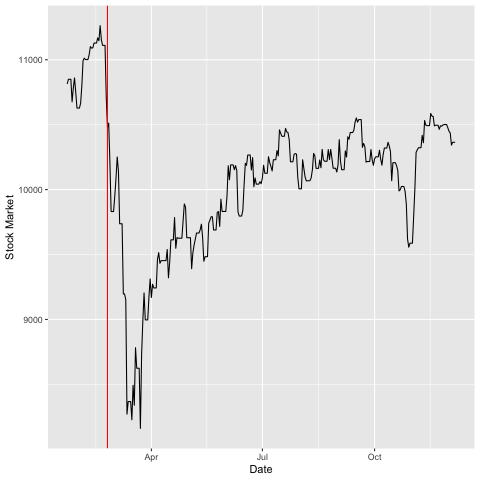
\includegraphics[width=100mm]{R-Code/plots/switzerlandFinance.png} \\
\caption{Switzerland stock market and first confirmed COVID-19 case}
\label{switzerland-covid-market}
\end{figure}

Figure \ref{switzerland-covid-numbers} shows how the numbers of COVID-19 infections and deaths increased over time. The plot indicates that Switzerland is currently in its second wave of infections. The same can be said for Germany and Italy. The plot for the USA indicates that they have not coped with the first wave yet. The plot for China shows that they have very few infections after the first wave.

\begin{figure}[!h]
\centering
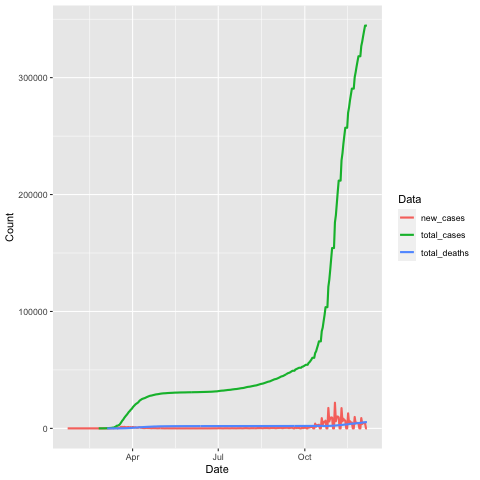
\includegraphics[width=100mm]{R-Code/plots/switzerlandCovid.png} \\
\caption{Switzerland COVID-19 data}
\label{switzerland-covid-numbers}
\end{figure}




\subsubsection{Datapreparation: Returns}
In the financial sector, in addition to the absolute level of a time series, its growth rates/returns are often of interest.
Since continuous growth rates/returns are additive due to logarithmizing and more closely match the normal distribution, they are often preferred to discrete returns in time series analysis and econometrics in general. (\cite{PowerPoi49:online})
$$r_{t} =\ln \left(Y_{t}\right)-\ln \left(Y_{t-1}\right)$$

\subsection{Stationarity}
In order to create the VAR models, we must first ensure that the time series are stationary. "A stationary time series is one whose statistical properties such as mean, variance, autocorrelation, etc. are all constant over time."(\cite{Stationa72:online}) For verification, the Augemented Dicky Fullman test is performed on all time series. The test returns the following p-values for the corona case numbers per country:
\begin{table}[H]
\centering
\caption{P-Values }
\label{tab:p-values-corona}
\begin{tabular}{|l|l|l|l|}
\hline
\textbf{Country} &  \textbf{P-Value Corona Cases} & \textbf{P-Value Corona Deaths} & \textbf{P-Value Financial Market} \\ \hline
China            & 0.01 & 0.01 & 0.33            \\ \hline
Italy            & 0.01 & 0.01 & 0.41           \\ \hline
Switzerland      & 0.99 & 0.44 & 0.26          \\ \hline
Germany          & 0.96 & 0.28  & 0.55          \\ \hline
USA              & 0.99 & 0.01  & 0.38        \\ \hline
\end{tabular}
\end{table}
The time series where the P-value is greater than 0.05 are not stationary. Therefore we try to create stationarity by using the first differences. Since the $log(0)$ is not defined and the corona time series have entries matching zero, we only use the \lstinline{diff()} function and  not the \lstinline{diff(log())} function. For the financial data, the \lstinline{diff(log())} is used.
\begin{table}[h!]
\centering
\caption{P-Values after first Differences}
\label{tab:p-values-first-diff}
\begin{tabular}{|l|l|l|l|}
\hline
\textbf{Country} &\textbf{P-Value Corona Cases} & \textbf{P-Value Corona Deaths} & \textbf{P-Value Financial Market}  \\ \hline
China            & - & - & 0.01            \\ \hline
Italy            & - & - & 0.01          \\ \hline
Switzerland      & 0.95 & 0.99 & 0.01           \\ \hline
Germany          & 0.99 & 0.99 & 0.01           \\ \hline
USA              & 0.99 & -  & 0.01         \\ \hline
\end{tabular}
\end{table}

\begin{table}[h!]
\centering
\caption{P-Values after second Differences}
\label{tab:p-values-second-diff}
\begin{tabular}{|l|l|l|}
\hline
\textbf{Country} &\textbf{P-Value Corona Cases} & \textbf{P-Value Corona Deaths}  \\ \hline
Switzerland      & 0.01 & 0.01         \\ \hline
Germany          & 0.01 & 0.01             \\ \hline
USA              & 0.01 & -            \\ \hline
\end{tabular}
\end{table}

\subsection{VAR-Modell and Granger Causality}
After ensuring the stationarity of the time series by applying first and second differences, the next phase is to apply the VAR model to the stationary time series. The VAR models explains one variable linearly with both their own previous values and through the previous values of other endogenous variables.(\cite{PowerPoi49:online}) A VAR model with three explanatory variables is calculated, as we analyse the three time series Corona cases, Corona deaths and financial markets.

A VAR model with 3 variables $X_{t},Y_{t}, Z_{t}$ and $lag = 1$:
$$
\begin{array}{l}
Y_{t}=a_{1}+\beta_{11} Y_{t-1}+\beta_{12} X_{t-1}+\beta_{13} Z_{t-1}+\epsilon_{1, t} \\
X_{t}=a_{2}+\beta_{21} X_{t-1}+\beta_{22} Y_{t-1}++\beta_{23} Z_{t-1}\epsilon_{2, t}\\
Z_{t}=a_{1}+\beta_{31} Z_{t-1}+\beta_{32} X_{t-1}++\beta_{33} Y_{t-1}\epsilon_{3, t}
\end{array}
$$

The $ lag = $ is determined using of the Akaike Index.
% --------------------
\section{Results}
% --------------------
% --------------------
\subsection{Outlook}
% --------------------



\section{Appendix}

% Finance plots
\begin{figure}[h!]
\centering
  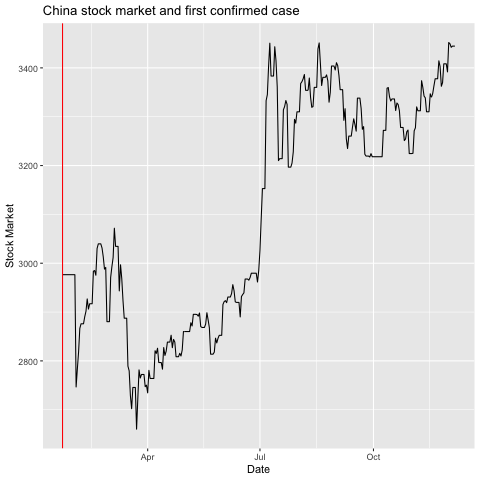
\includegraphics[width=100mm]{R-Code/plots/chinaFinance.png} 
  \caption{China stock market and first confirmed COVID-19 case}
  \label{china-covid-market}
\end{figure}

\begin{figure}[!h]
\centering
  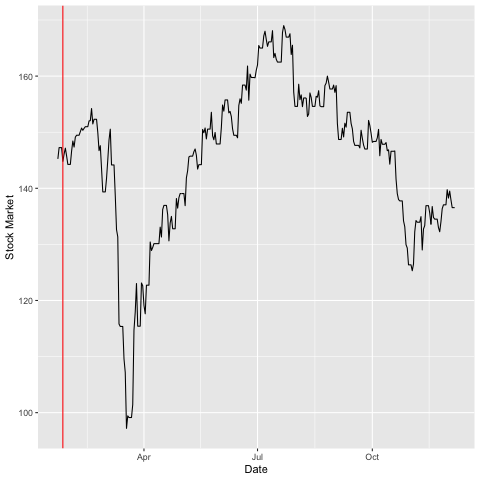
\includegraphics[width=100mm]{R-Code/plots/germanyFinance.png}   
  \caption{Germany stock market and first confirmed COVID-19 case}
  \label{germany-covid-market}
\end{figure}

\begin{figure}[!h]
\centering
  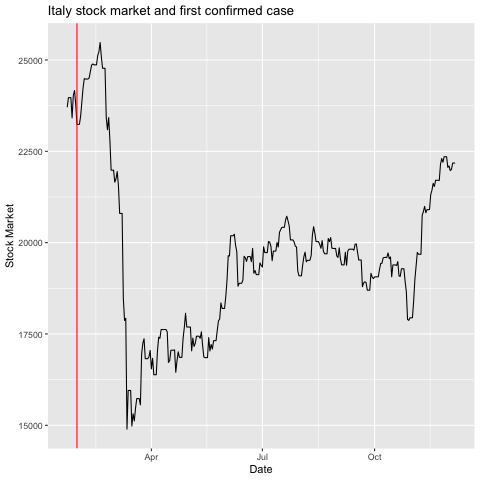
\includegraphics[width=100mm]{R-Code/plots/italyFinance.png}  
  \caption{Italy stock market and first confirmed COVID-19 case}
  \label{italy-covid-market}
\end{figure}

\begin{figure}[!h]
\centering
  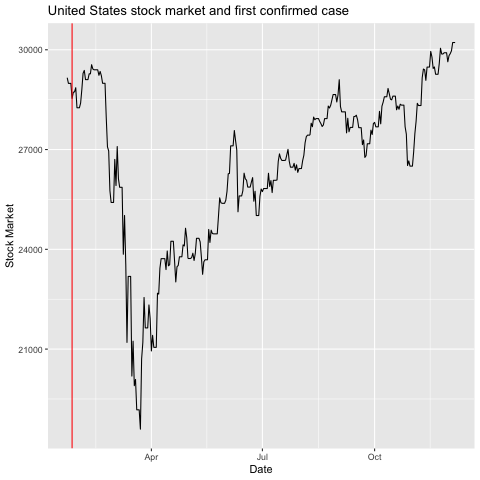
\includegraphics[width=100mm]{R-Code/plots/usaFinance.png} 
    \caption{USA stock market and first confirmed COVID-19 case}
    \label{usa-covid-market}
\end{figure}

% Covid Plots
\begin{figure}[h!]
\centering
  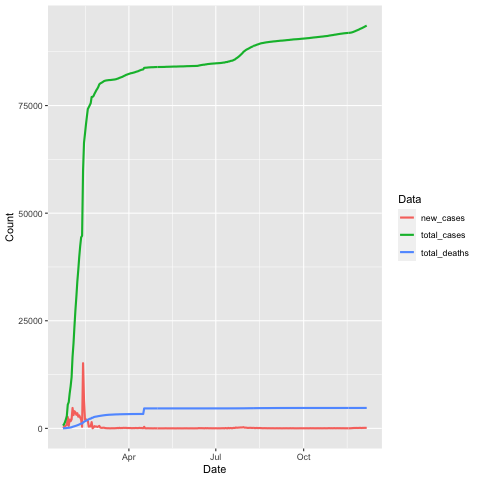
\includegraphics[width=110mm]{R-Code/plots/chinaCovid.png} 
  \caption{China COVID-19 data}
\end{figure}

\begin{figure}[!h]
\centering
  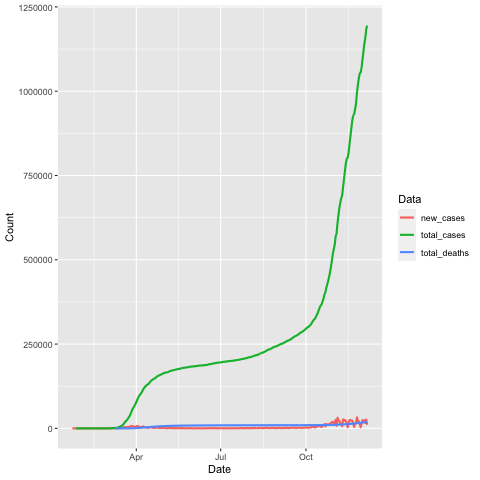
\includegraphics[width=110mm]{R-Code/plots/germanyCovid.png}   
  \caption{Germany COVID-19 data}
  \end{figure}

\begin{figure}[!h]
\centering
  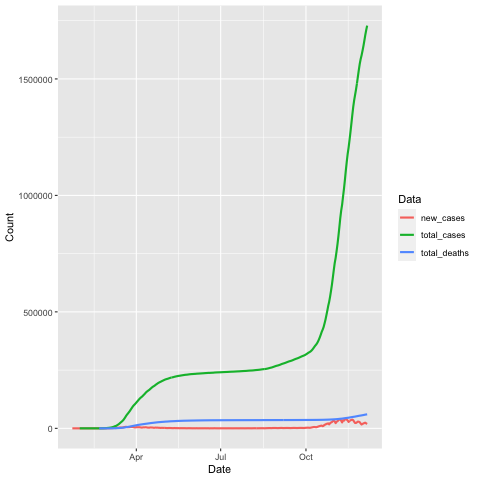
\includegraphics[width=110mm]{R-Code/plots/italyCovid.png}  
  \caption{Italy COVID-19 data}
  \end{figure}

\begin{figure}[!h]
\centering
  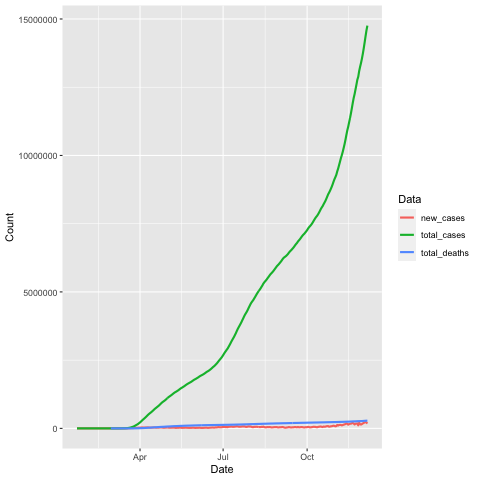
\includegraphics[width=110mm]{R-Code/plots/usaCovid.png} 
  \caption{United States COVID-19 data}
\end{figure}

% %%%%%%%%%%%%%%%%%%%%%%%%%%%%%%%%%%%%%%%%%%%%%%%%%%%%%%%%%%
% %%%%%%%%%%%%%%%%%%%%%%%%%%%%%%%%%%%%%%%%%%%%%%%%%%%%%%%%%%
% REFERENCES SECTION
% %%%%%%%%%%%%%%%%%%%%%%%%%%%%%%%%%%%%%%%%%%%%%%%%%%%%%%%%%%
% %%%%%%%%%%%%%%%%%%%%%%%%%%%%%%%%%%%%%%%%%%%%%%%%%%%%%%%%%%
\clearpage
\medskip
\newpage

\nocite{*} 
\bibliography{references.bib} 

\end{document}